%%%%%%%%%%%%%%%%%%%%%%%%%%%%%%%%%%%%%%%%%
% Short Sectioned Assignment
% LaTeX Template
% Version 1.0 (5/5/12)
%
% This template has been downloaded from:
% http://www.LaTeXTemplates.com
%
% Original author:
% Frits Wenneker (http://www.howtotex.com)
%
% License:
% CC BY-NC-SA 3.0 (http://creativecommons.org/licenses/by-nc-sa/3.0/)
%
%%%%%%%%%%%%%%%%%%%%%%%%%%%%%%%%%%%%%%%%%

%----------------------------------------------------------------------------------------
%	PACKAGES AND OTHER DOCUMENT CONFIGURATIONS
%----------------------------------------------------------------------------------------

\documentclass[paper=a4, fontsize=11pt]{scrartcl} % A4 paper and 11pt font size

\usepackage[T1]{fontenc} % Use 8-bit encoding that has 256 glyphs
%\usepackage{fourier} % Use the Adobe Utopia font for the document - comment this line to return to the LaTeX default
\usepackage[english]{babel} % English language/hyphenation
\usepackage{amsmath,amsfonts,amsthm} % Math packages

\usepackage{lipsum} % Used for inserting dummy 'Lorem ipsum' text into the template

\usepackage{sectsty} % Allows customizing section commands
\allsectionsfont{\centering \normalfont\scshape} % Make all sections centered, the default font and small caps

\usepackage{fancyhdr} % Custom headers and footers
\pagestyle{fancyplain} % Makes all pages in the document conform to the custom headers and footers
\fancyhead{} % No page header - if you want one, create it in the same way as the footers below
\fancyfoot[L]{} % Empty left footer
\fancyfoot[C]{} % Empty center footer
\fancyfoot[R]{\thepage} % Page numbering for right footer
\renewcommand{\headrulewidth}{0pt} % Remove header underlines
\renewcommand{\footrulewidth}{0pt} % Remove footer underlines
\setlength{\headheight}{13.6pt} % Customize the height of the header

\numberwithin{equation}{section} % Number equations within sections (i.e. 1.1, 1.2, 2.1, 2.2 instead of 1, 2, 3, 4)
\numberwithin{figure}{section} % Number figures within sections (i.e. 1.1, 1.2, 2.1, 2.2 instead of 1, 2, 3, 4)
\numberwithin{table}{section} % Number tables within sections (i.e. 1.1, 1.2, 2.1, 2.2 instead of 1, 2, 3, 4)

\setlength\parindent{0pt} % Removes all indentation from paragraphs - comment this line for an assignment with lots of text

%----
%%Custom packages
%----
\usepackage{graphicx}

%----------------------------------------------------------------------------------------
%	TITLE SECTION
%----------------------------------------------------------------------------------------

\newcommand{\horrule}[1]{\rule{\linewidth}{#1}} % Create horizontal rule command with 1 argument of height

\title{	
\normalfont \normalsize 
\textsc{Technische Universität München, Lehrstuhl für Elektrische Antriebe und Leistungselektronik} \\ [25pt] % Your university, school and/or department name(s)
\horrule{0.5pt} \\[0.4cm] % Thin top horizontal rule
\huge Praktikum: Systemidentifikation eines nichtlinearen Schwingungssystems \\ % The assignment title
\horrule{2pt} \\[0.5cm] % Thick bottom horizontal rule
}

\author{Maximilian Schermer, Matrikelnummer: 03664650, \\ Maximilian Sperr, Matrikelnummer: 03658841,\\ Giulio Evangelisti,  Matrikelnummer: 03659301} % Your name

\date{\normalsize\today} % Today's date or a custom date

\begin{document}

\maketitle % Print the title

%----------------------------------------------------------------------------------------
%	PROBLEM 1
%----------------------------------------------------------------------------------------
%\newpage

\section{Duffing Oszillator}

\subsection{Systembeschreibung}

Unser gewähltes System lässt sich im inhomogenen, erzwungenem Fall durch folgende nichtlineare Differentialgleichung darstellen \cite{Duffing}:
\begin{equation}
\ddot{q}+\delta \dot{q}+\alpha q+\beta q^3=u(t)=\gamma \cos(\omega_d t)\, .
\end{equation}

Es lässt sich daher als Erweiterung des allgemein bekannten gedämpften Oszillatormodells um den kubischen Rückstellterm $\beta q^3$ interpretieren. Daher entspricht $\delta$ der linearen Dämpfung, $\alpha=\omega_0^2$ der um die Masse oder Massenträgheit normierte lineare Term der rücktreibenden Kraft mit der natrürlichen Eigenfrequenz $\omega_0=2\pi f_0$, während $\gamma$ und $\omega_d$ Amplitude und Frequenz der antreibenden Sinusschwingung darstellen.

\subsection{Praxisbezug}

Die Bedeutung von Schwingungssystemen in der Natur ist unbestreitbar. Eine durchgehend lineare Rückstellkraft nach dem Hook'schen Gesetz $F=-kq$ ist allerdings nur idealisiert zutreffend für die meisten Systeme, deren Gültigkeit beschränkt ist auf kleine Amplituden. Durch die strukturelle Zusammensetzung des Schwingers nimmt diese rücktreibende Kraft entweder (auf nichtlineare Art und Weise) zu oder ab. Dies wird (in 1. Ordnung) durch den nach George Duffing benannten Duffing-Term $\beta q^3$ modelliert.\\
Beispiele für Schwingungssysteme, die sich sehr gut als Duffing System mathematisch beschreiben lassen, sind sämtliche Schwingungssysteme, die nichtlineare Eigenschaften wie eine veränderliche Eigenfrequenz, chaotisches Verhalten, Bifurkation, etc. zeigen \cite{Duffing}, wie z.B. konkret ein Pendel mit einer Unwucht oder ein Feder-Masse-System mit einer sog. "hardening spring" ($\beta>0$) \cite{Khalil}.

\subsection{Simulationen}

Mit Simulationen wird das stark nichtlineare Verhalten des Systems untersucht.
Dessen chaotisches Verhalten lässt sich besonders gut veranschaulichen durch Variation der Amplitude $\gamma$ der antreibenden Schwingung (vgl. Fig.~\ref{gammas}). Hier sind im oberen Plot die Phasenportraits mit den Zuständen $x_1=q$, $x_2=\dot{q}$, im mittleren die zeitliche Schwingung $x_1(t)=q(t)$, und im untersten Plot der approximierte Frequenzgang des Systems, mit der normierten steady-state Amplitude $z/\gamma$ für die jeweils unterschiedlichen Paramterwerte dargestellt.

\begin{figure}[!h]
	\centering
		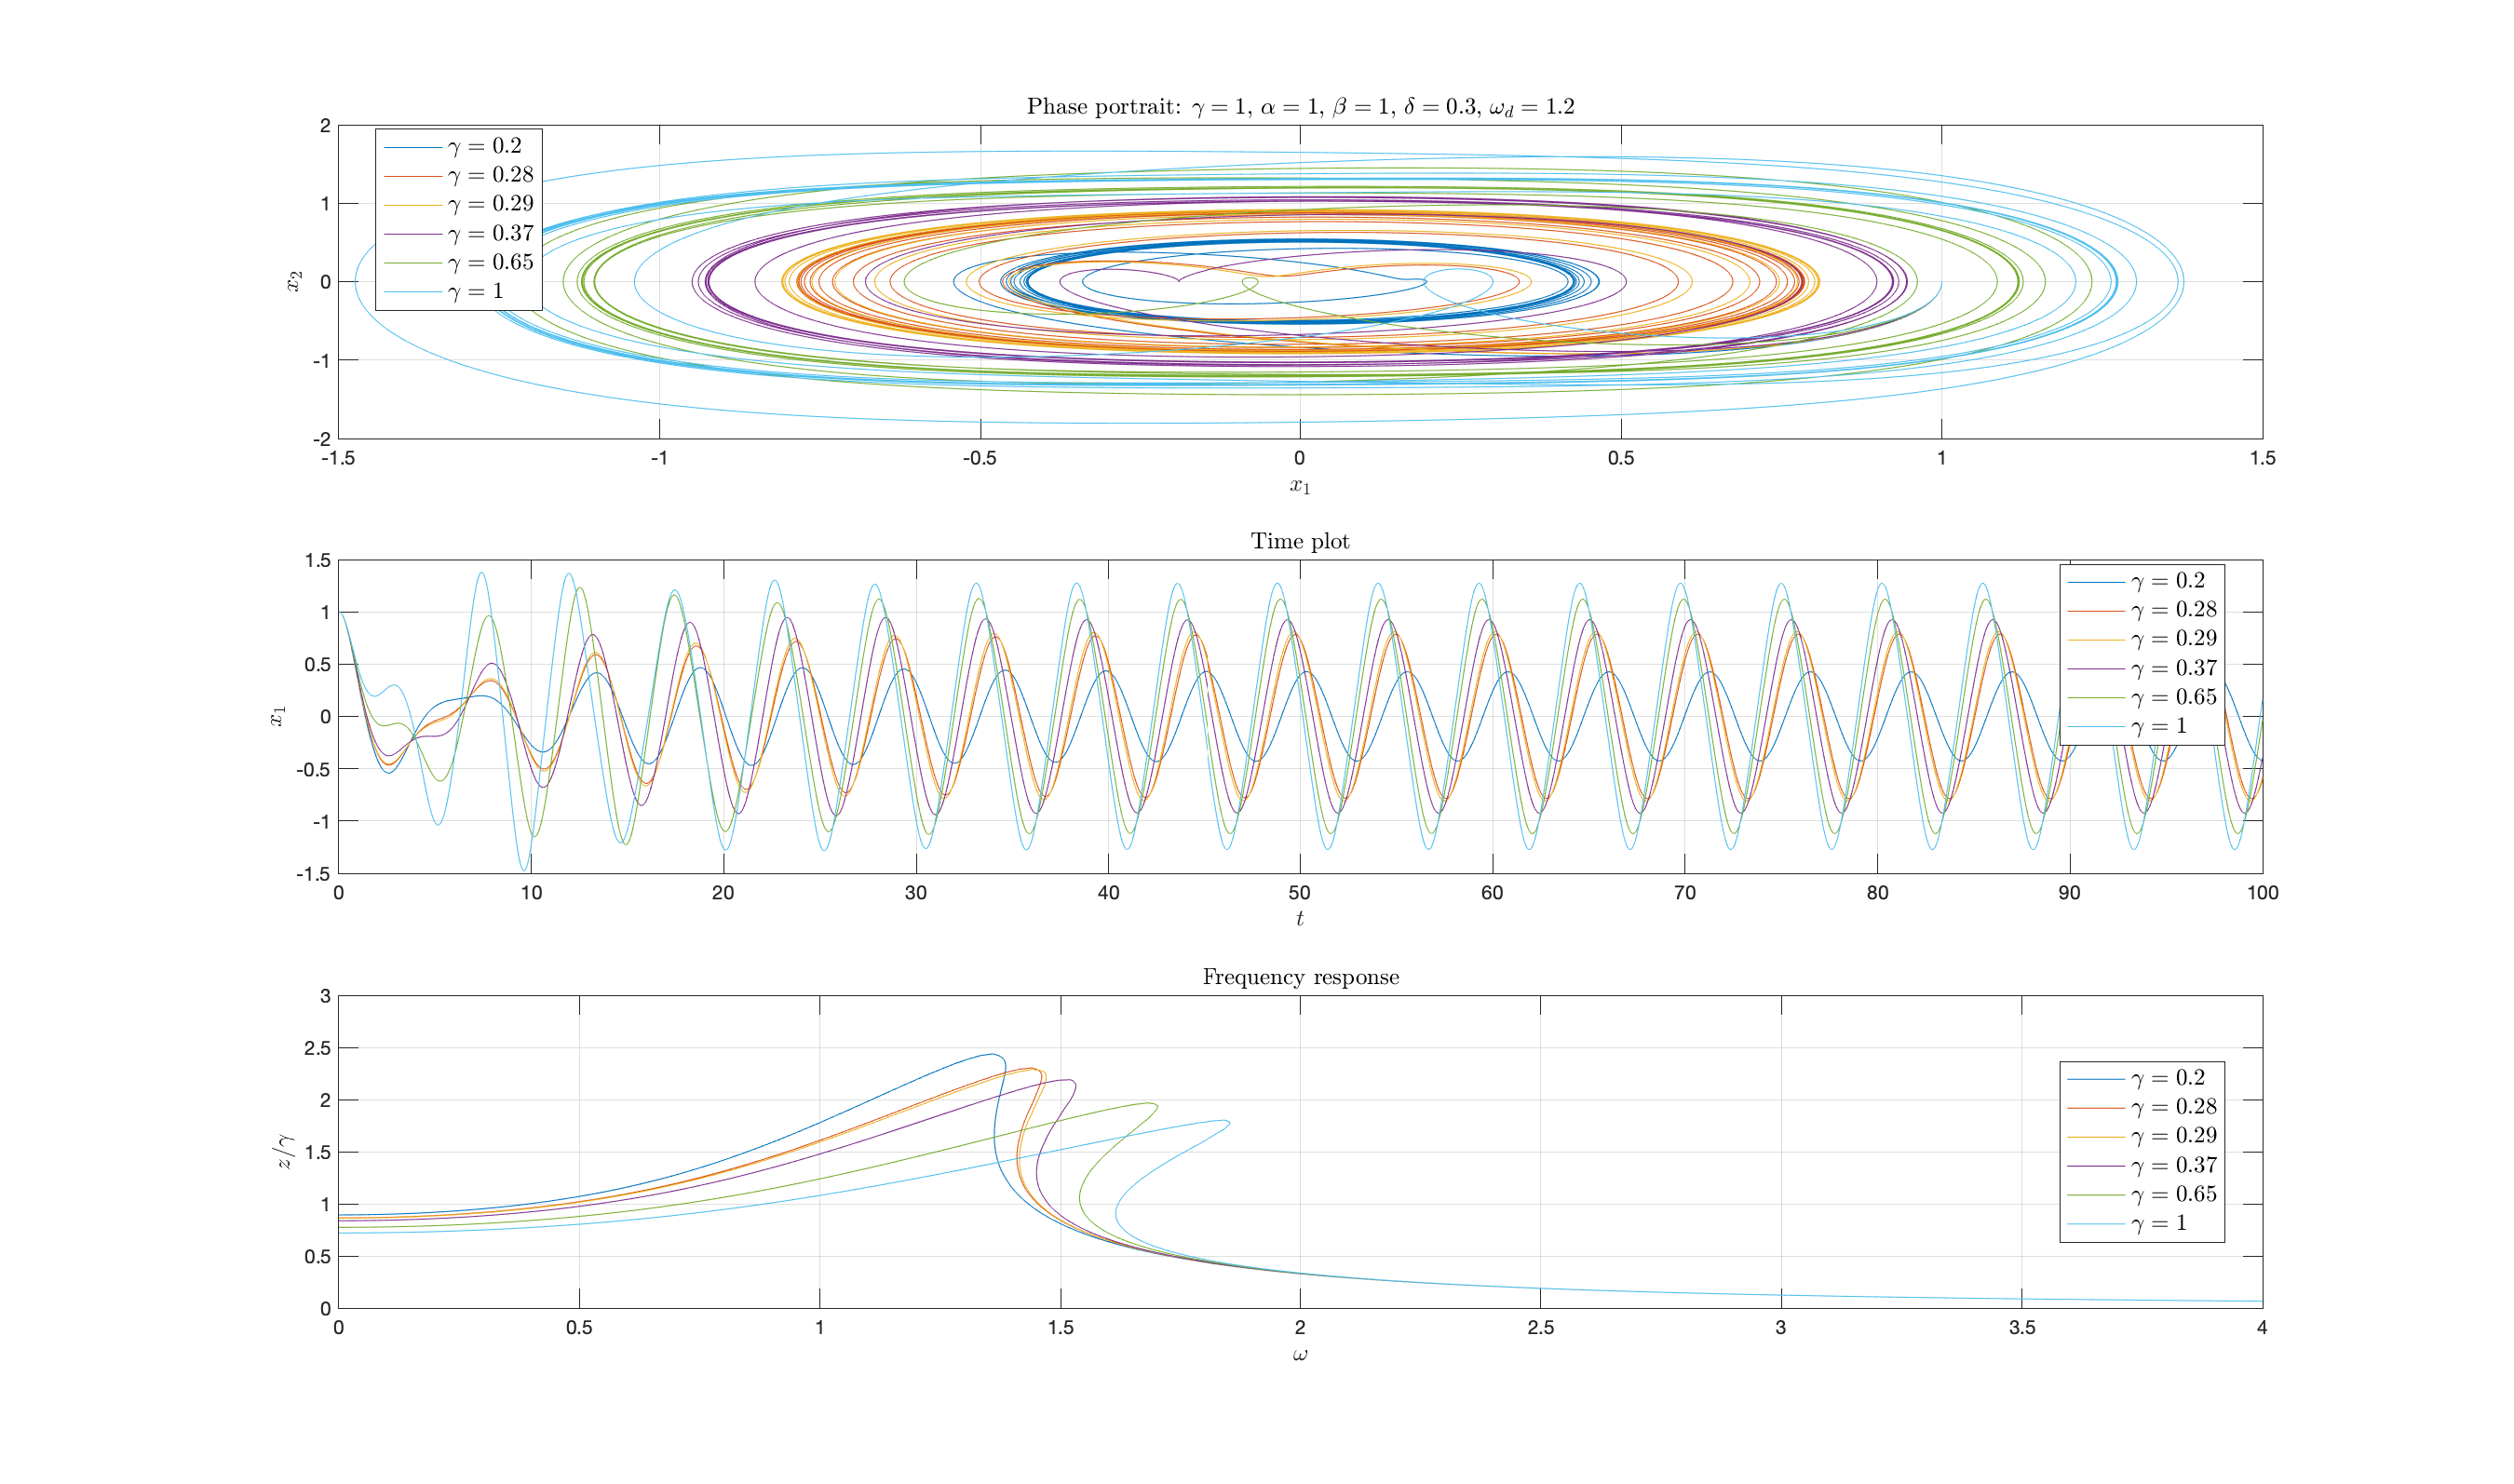
\includegraphics[width=1\textwidth]{./gammas.eps}
	\caption{Simulation des Duffing Systems für unterschiedliche Anregungsamplituden. Die restlichen Parameter wurden gewählt als $\delta=0.3$, $\alpha=1$, $\beta=1$, $\omega_d=1.2$ sowie die Anfangsbedinungen zu $x_1(0)=1$ und $x_2(0)=0$.}
	\label{gammas}
\end{figure}

Eine Simulation der Strecke mit unseren von nun an verwendeten Parameterwerten ist abgebildet in Fig.~\ref{plant}.

\begin{figure}[!h]
	\centering
		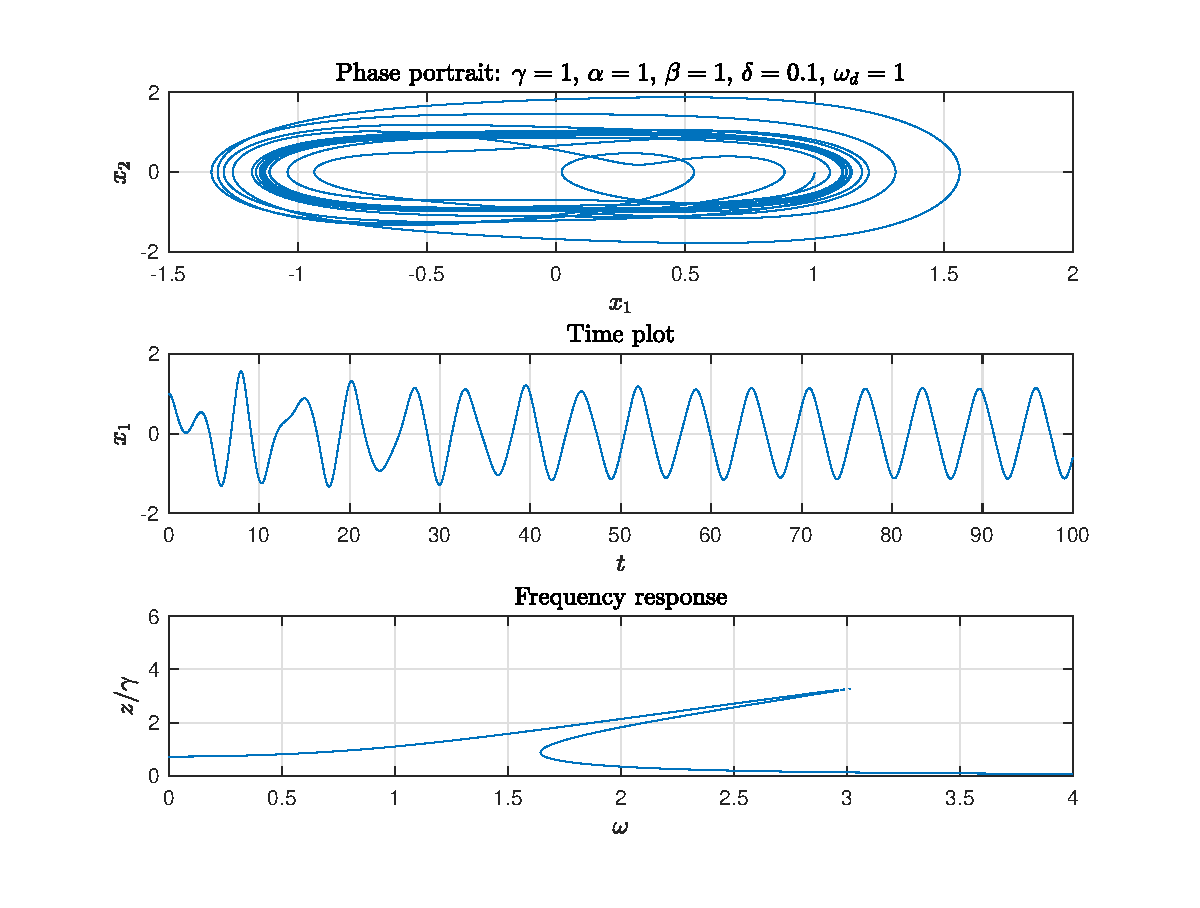
\includegraphics[width=1\textwidth]{./plant_sim.eps}
	\caption{Simulation mit unserem ausgewählten Parametersatz: $\gamma=1$, $\delta=0.1$, $\alpha=1$, $\beta=1$, $\omega_d=1$ sowie $x_1(0)=1$ und $x_2(0)=0$.}
	\label{plant}
\end{figure}

%------------------------------------------------

\section{Identifikationsmodell}\label{Identifikationsmodell}

Als Identifikationsmodell dient das General Dynamic Neuronal Network (GDNN) welches aus drei versteckten Schichten mit zweimal zwei und einmal einem Neuron (2-2-1) besteht. In der Eingangs sowie in der Ausgangsschicht befindet sich ein Neuron und die verschiedenen Schichten sind miteinander über Tapped Delay Lines gekoppelt. Die Tapped Delay Lines sind wie folgt aufgebaut:

\begin{table}[!h]
	\centering
		\begin{tabular}{*{3}{p{4cm}}}
			Schicht 1 & Schicht 2 & Schicht 3 \\
			$DI^{1,1} =  \left\{1,2,3\right\}$ & $DL^{2,1} =  \left\{0\right\}$ & $DL^{3,2} =  \left\{0\right\}$ \\
			$DL^{1,1} =  \left\{1,2,3\right\}$ & $DL^{2,2} =  \left\{1,2,3\right\}$ & $DL^{3,3} =  \left\{1,2,3\right\}$ \\
			$DL^{1,2} =  \left\{1,2,3\right\}$ & $DL^{2,3} =  \left\{1,2,3\right\}$ \\
			$DL^{1,3} =  \left\{1,2,3\right\}$ \\			
		\end{tabular}
\end{table}

Die Identifikation findet mittels eines NARX Modells statt, d.h. der Systemausgang und das Anregungssignal sind die Eingänge für das neuronale Netz. Das GDNN wurde wegen seiner hohen Approximationsfähigkeit ausgewählt. 

Im folgenden wurde die zur Verfügung gestellte Identifikationssoftware GDNN Version A verwendet.
%------------------------------------------------

\section{Systemanregung}

%Anregungssignal beschrieben, Grund für Chirp angeben, Frequenzabhängigkeit des Systems.
Wegen der starken Frequenzabhängigkeit unseres Systems, kann dieses nicht mit einem APRBS-Signal angeregt werden. Dies würde zu Amplitudenschwankungen des Systems führen welche den Lernprozess stören. Aus diesem Grund werden als Anregungssignal zwei Chirp Signale miteinander verbunden. Das erste Chirp Signale hat eine steigende Frequenz $\left[0; \frac{2}{\pi}\right]$ und das zweite eine abfallende Frequenz $\left[\frac{2}{\pi};0\right]$. Somit wird gewährleistet, dass alle Frequenzen bzw. Kreisfrequenzen $\left[0;4\right]$ der Frequenzantwort durchlaufen werden.
\begin{figure}[!h]
	\centering
		\includegraphics[width=0.9\textwidth]{./AnregungChirp.png}
	\caption{Anregungssignal}
	\label{fig:AnregungChirp}
\end{figure}
\newpage
%------------------------------------------------

\section{Identifikationsergebnisse}

%Identifikationsergebnis, Validierung Modell
Der Lernprozess wird über 100$s$ ausgeführt. Dabei ergeben sich folgende Identifikationsergebnisse:
Obwohl das System sehr starke Nichtlinearitäten aufweist, erzielen wir gute Identifikationsergebnisse bis zu einem Fehler von $10^{-6}$. Dieses Ergebnis ist zufriedenstellend. Anfangs kommt es zu starken Abweichung, da der Lernprozess nicht weit fortgeschritten ist.
\begin{figure}[!h]
	\centering
		\includegraphics[width=1.00\textwidth]{./Q_500_nice_results_double_chirp.png}
	\caption{Anregungssignal, Ausgang System, Ausgang Modell}
	\label{fig:Nice_result_double_chirp}
\end{figure}

\begin{figure}[!h]
	\centering
		\includegraphics[width=0.5\textwidth]{./Q_500_nice_results_double_chirp_2.png}
	\caption{Verlauf des Fehlers}
	\label{fig:Nice_result_double_chirp2}
\end{figure}
\newpage

Eine erneute Identifikation über 80$s$ mit darauffolgender Validierung über 20$s$, bei der der Lernprozess abgeschaltet wird, ergab folgende Ergebnisse: 
\begin{figure}[!h]
	\centering
		\includegraphics[width=1.00\textwidth]{./Q_500_nice_results_double_chirp_validierung_80.png}
	\caption{Anregungssignal, Ausgang System, Ausgang Modell mit Validierung nach 80s}
	\label{fig:Validierung}
\end{figure}

\begin{figure}[!h]
	\centering
		\includegraphics[width=0.5\textwidth]{./Q_500_nice_results_double_chirp_validierung_80_2.png}
	\caption{Verlauf des Fehlers mit Validierung nach 80s}
	\label{fig:Validierung2}
\end{figure}

Die Ergebnisse zeigen, dass der Fehler nach abschalten des Lernens zwar ansteigt, aber die Identifikation weiterhin gute Resultate liefert.
\newpage
%------------------------------------------------

\section{Anpassung des Identifikationsmodells}

%Modellstruktur und Anregungssignal ändern. Zu statischen Identifikationsmodell wechseln.
\subsection{Änderung Modellstruktur}
Wird die Modellstruktur so abgewandelt, dass keine zeitliche Verzögerungen (TDL) zwischen den Schichten existieren und die Rückführungen bestehen bleiben, so ergeben sich folgende Ergebnisse:
\begin{figure}[!h]
	\centering
		\includegraphics[width=1.00\textwidth]{./GDNN_ohneTDL_Identifikation.png}
	\caption{Anregungssignal, Ausgang System, Ausgang Modell mit GDNN ohne TDL}
	\label{fig:GDNN_ohneTDL}
\end{figure}

\begin{figure}[!h]
	\centering
		\includegraphics[width=0.5\textwidth]{./GDNN_ohneTDL_Identifikation_2.png}
	\caption{Verlauf des Fehlers mit GDNN ohne TDL}
	\label{fig:GDNN_ohneTDL2}
\end{figure}
\newpage

\subsection{Änderung Anregungssignal}
Eine Änderung des Anregungssignals auf ein klassisches APRBS Signal erzeugt den bereits schon angesprochene schlechten Lernprozess. Die Modellstruktur entspricht wieder der Struktur des zu Anfang angesprochene GDNN-Modells.
\begin{figure}[!h]
	\centering
		\includegraphics[width=1.00\textwidth]{./APRBS_GDNN.png}
	\caption{Anregungssignal, Ausgang System, Ausgang Modell mit APRBS-Signal}
	\label{fig:APRBS}
\end{figure}

\begin{figure}[!h]
	\centering
		\includegraphics[width=0.5\textwidth]{./APRBS_GDNN_2.png}
	\caption{Verlauf des Fehlers mit APRBS-Signal}
	\label{fig:APRBS2}
\end{figure}
\newpage

\subsection{Änderung auf statisches Modell (MLP)}
Eine Änderung des Modells auf ein statisches Modell welches einem MLP entspricht, liefert ebenfalls einen schlechten Lernprozess. Dies liegt vor allem daran, dass das MLP die starke Nichtlinearität des Duffing Systems nicht identifizieren kann.
\begin{figure}[!h]
	\centering
		\includegraphics[width=1.00\textwidth]{./MLP_Identifikation.png}
	\caption{Anregungssignal, Ausgang System, Ausgang Modell mit MLP-Modell}
	\label{fig:MLP}
\end{figure}

\begin{figure}
	\centering
		\includegraphics[width=0.5\textwidth]{./MLP_Identifikation_2.png}
	\caption{Verlauf des Fehlers mit MLP-Modell}
	\label{fig:MLP2}
\end{figure}

\bibliography{ref}
\bibliographystyle{plainurl}

\end{document}